% %!TEX root = main.tex
\subsection{The Microsoft Kinect SDK}


\begin{frame}
\frametitle{Data streams}

\begin{figure*}[ht!]
  \centering
  \begin{minipage}{0.32\textwidth}
  	\centering
    \includegraphics[width=\textwidth]{figs/color-frame}\\
    Color Stream
  \end{minipage}\hfill
  \begin{minipage}{0.32\textwidth}
  	\centering
	\includegraphics[width=\textwidth]{figs/depth-frame}\\
    Depth Stream
  \end{minipage}\hfill
  \begin{minipage}{0.32\textwidth}
  	\centering
    \includegraphics[width=\textwidth]{figs/skeleton-frame}\\
    Skeleton Stream
  \end{minipage}
\end{figure*}

\end{frame}


\begin{frame}
\frametitle{Skeleton Joints}
\begin{itemize}
\item A total of 20 inferred joints
\item Organized in a hierarchical structure (we make use of this later)
\end{itemize}

\begin{figure*}[ht!]
\label{fig1}
\centering
\begin{minipage}{0.34\linewidth}
\centering
\includegraphics[width=\linewidth]{figs/skeleton.pdf}\\
Skeletal Joints
\end{minipage}\hfill
\begin{minipage}{0.6\linewidth}
\centering
\resizebox{\linewidth}{!} {
\tikzset{edge from parent/.style=
{draw, edge from parent path={(\tikzparentnode.south)
-- +(0,-3pt)
-| (\tikzchildnode)}},
blank/.style={draw=none}}
    \begin{tikzpicture}

    \node{\Tree 
     [.{HipCenter} 
        [.Spine [.{Shoulder Center}  [.{Shoulder Left} [.{Elbow Left} [.{Wrist Left} [.{Hand Left} ]]]]  {Head} [.{Shoulder Right} [.{Elbow Right} [.{Wrist Right} [.{Hand Right} ]]]]  ]]
        [.{Hip Left} [.{Knee Left} [.{Ankle Left} [.{Foot Left} ]]]]
        [.{Hip Right} [.{Knee Right} [.{Ankle Right} [.{Foo tRight} ]]]]
        ]};
    \end{tikzpicture}
}\\
Joints in a tree structure
\end{minipage}

\end{figure*}
\end{frame}
